\chapter{Alkalmazások}

A kapcsolási rajz és a nyáktervezés során fontos szempontok voltak, hogy univerzális legyen az áramkör és könnyen lehessen integrálni már meglévő megoldásokkal. A különböző alkalmazások során felmerülő igények érdekében ugyanaz az áramkör használható a felhasználói oldalon az irányításhoz, mint például a beavatkazó oldalhoz. Ez azért valósítható meg, mert elegendő néhány alapvető elemen kívűl csak a használathoz specifikus alkatrészek beültetése.
A következőkben lehetséges konfigurációkat mutatok be, illetve hogy az adott konfigurációkat milyen alkalmazások tudják használni.

\section{Elérhető perifériák}
Az áramkör tervezése során az alábbi szenzorok, illetve egyéb perifériákkal való kompatibilitás volt figyelembe véve. Ezek különböző kombinációja alkot egy konfigurációt, amiről a későbbiekben lesz szó. A listában zárójelben látható továbbá, hogy az adott eszköz használatához milyen és hány darab elérhető csatlakoztatási pontra van szükség. Néhány eszköz esetében számít sebesség, ezért ezeket közvetlenül a mikrokontroller lábaira szükséges kötni.
\begin{itemize}
    \item 7 db GPIO láb
    \item 1 db 16 bites shift regiszter ( 16 db be vagy kimenet)
    \item 1 db 8 bites párhuzamos kimenetnel rendelkező shift regiszter ( 3db kimenet )
    \item 1 db 8 bites párhuzamos bemenettel rendelkező shift regiszter ( 3db kimenet )
    \item OLED kijelző ( I2C )
    \item Enkóder nyomógombbal ( 3 db bemenet )
    \item 4 db N csatornás MOSFET-tel vezérelt meghajtó ( 4 db kimenet)
    \item 2 db P csatornás MOSFET-tel vezérelt meghajtó ( 2 db kimenet)
    \item 2 db N csatornás MOSFET-tel megvalósított bemenet ( 2db bemenet )
    \item IR Adó / Vevő ( 1 db kimenet, 1 db bemenet)
    \item Mozgásérzékelő ( 1 db bemenet)
    \item Optokapuk ( 2db kimenet )
    \item Hőmérséklet szenzor ( I2C )
    \item ADC ( 1 db analóg bemenet )
    \item 7 szegmenses kijelző modul ( 2 db kimenet )
    \item RGB LED ( 1 db kimenet )
    \item Normál LED ( 1 db kimenet )
\end{itemize}

\begin{figure}[th!]
    \centering
    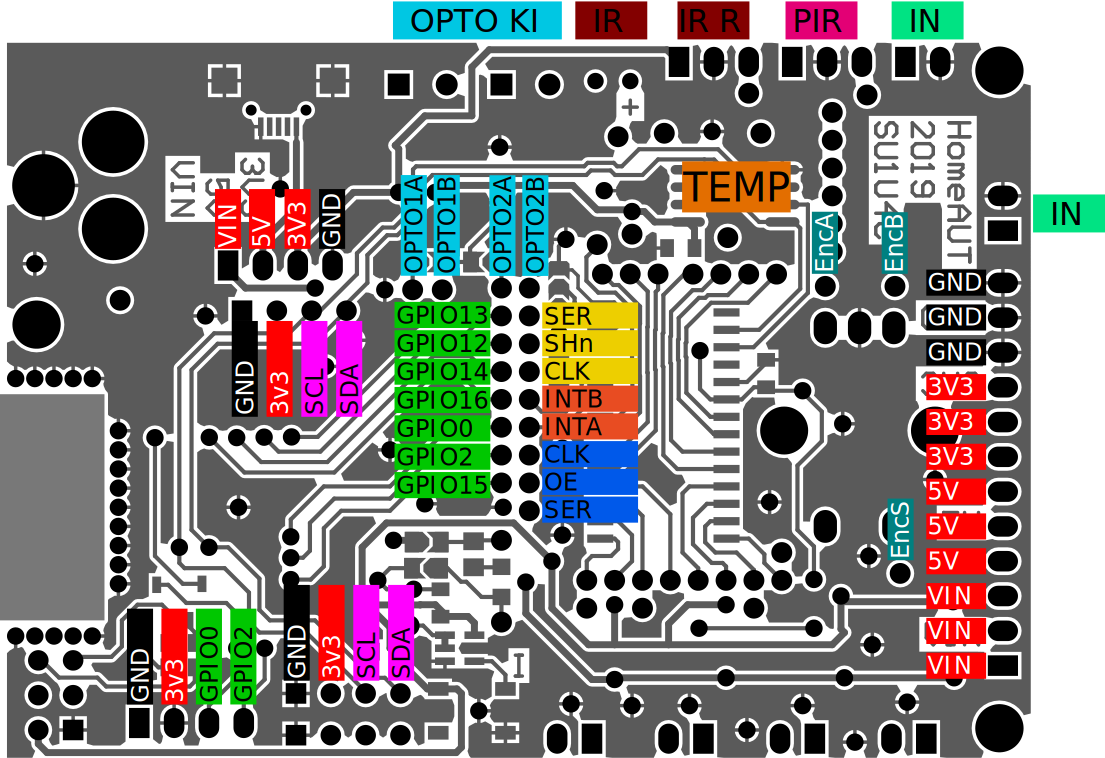
\includegraphics[width=150mm, keepaspectratio]{figures/board_bottom.pdf}
    \caption{Gyakran használt konfigurációs pontok}
    \label{fig:nodered_ui}
\end{figure}


\section{Konfigurációk}
Az elérhető perifériák lista alapján összeállítható egy táblázat \ref{tab:applications}, amelyről leolvasható, hogy milyen alkatrészeket tudunk egyszerre használni. A táblázat első sora ezeket az eszközöket tartalamazza. Minden eszközhöz továbbá felvan tüntetve, hogy hány láb szükséges a működéshez. Az első oszlop tartalmazza a mikrokontroller elérhető lábait, illetve használható shift regisztereket. Külön megjegyzésben található, ha az adott lábnak van plusz funkciója, illetve ha a boot mód kiválasztása miatt szükséges volt egy alapállapot beállítása. A táblázatban, ha egy alkatrész tudná használi az adott lábat, akkor az metszet x-el van jelölve

Két eszközt ezek alapján, akkor tudunk egyszerre használni, ha kitudunk választani úgy a lábakat, hogy a két oszlopban a megjelölt elemek között nincs átfedés átfedés. Figyelembe kell venni emelett, ha például a kijelző használja I2C interfészt, akkor ezzel nem zárja ki többi I2C-s eszközt. Ezeket az eszközöket i betű jelzi.
\afterpage{%
    \clearpage% Flush earlier floats (otherwise order might not be correct)
    \begin{landscape}% Landscape page
        \begin{table}[ht]
            \footnotesize
            \centering
            \begin{tabular}{r|ccccccccccccccccc}
                & \rot{SR 16 bit ki-bemenet} & \rot{SR 8 bit bemenet} & \rot{SR 8 bit kimenet} & \rot{OLED Kijelző} & \rot{Enkóder} & \rot{NFET kimenet} & \rot{NFET bemenet} & \rot{PFET kimenet} & \rot{IR adó ( direkt )} & \rot{IR vevő ( direkt )} & \rot{Mozgásérzékelő} & \rot{Optokapuk} & \rot{Hőmérséklet szenzor} & \rot{ADC} & \rot{7 szegmenses modul} & \rot{RGB LED} & \rot{LED}\\
                \hline
                \ &\\
                Szükséges lábak & I2C & 3 & 3 & I2C & 3 & max 4 & max 2 & max 2& 1 & 1 & 1 & max 2 & I2C & 1 & 2 & 1 & 1\\
                \ &\\
                GPIO0 (magas)          &   &   &   &   & x & x & x & x &   & x &   &   &   &   & x & x & x \\
                GPIO2 (magas)          &   &   &   &   & x & x & x & x &   & x &   &   &   &   & x & x & x \\
                GPIO15 (alacsony)      &   & x & x &   & x & x & x & x & x & x & x & x &   &   &   & x & x \\
                GPIO12                 &   & x & x &   & x & x & x & x & x & x & x & x &   &   & x & x & x \\
                GPIO13                 &   & x & x &   & x & x & x & x & x & x & x & x &   &   & x & x & x \\
                GPIO14                 &   & x & x &   & x & x & x & x & x & x & x & x &   &   & x & x & x \\
                GPIO16                 &   & x & x &   & x & x & x & x & x & x & x & x &   &   & x & x & x \\
                SR\_IN                 &   &   &   &   & x &   & x &   &   &   & x &   &   &   &   &   &   \\
                SR\_OUT                &   &   &   &   &   & x &   & x &   &   &   & x &   &   &   &   & x \\
                GPIO1 / Tx             &   &   &   &   &   &   &   &   &   &   &   &   &   &   &   &   &   \\
                GPIO3 / Rx             &   &   &   &   &   &   &   &   &   &   &   &   &   &   &   &   &   \\
                GPIO4 / SDA            & i & x & x & i & x & x & x & x & x & x & x & x & i &   & x & x & x \\
                GPIO5 / SCL            & i & x & x & i & x & x & x & x & x & x & x & x & i &   & x & x & x \\
                A0                     &   &   &   &   &   &   &   &   &   &   &   &   &   & x &   &   &   \\
                \hline
                \ &\\
                Példa konfigurációk \\
                A                      &   &   &   & x & x &   &   &   & x & x &   &   & x & x &   &   &   \\
                B                      &   &   &   &   &   & x & x &   & x &   & x &   & x &   &   &   &   \\
                C                      & x &   &   & x & x & x & x & x & x & x & x & x & x & x &   &   & x \\
                D                      &   &   &   &   & x & x &   &   &   &   &   & x & x & x &   &   &   \\
            \end{tabular}
            \caption{Lehetséges párosítások}
            \label{tab:applications}
        \end{table}
    \end{landscape}
    \clearpage% Flush page
}

\section{Példa alkalmazások}

Az "A" konfiguráció egy OLED kijelzőből, enkóderből, infra adóból és vevőből, hőmérséklet szenzorból és az ADC átalakítóból áll össze. Egy ilyen konfigurációval rendelkező eszközt lehet például termosztát vezérlőnek használni. A kijelző és enkóder segítségével könnyedén beállítható a kívánt hőmérséklet. Van rá lehetőség, hogy egyedi értékeket lehessen rendelni specifikus napszakokhoz. Az infra adó használatával lehetőség nyílik irányítani például már meglévő légkondicináló berendezést is. Szobánként elhelyezve ilyen egységeket az ESPNOW hálózat segítségével összetudnak kapcsolódni, hogy információt osszanak meg egymással és ezek alapján döntéseket hozni. Ilyen döntés lehet például az előbb említett légkondiciónálóval rendelkező szoba esetén, hogy alacsony hőmérséklet esetén kapcsolja be a központi fűtést vagy elegendő a légkondicionálóval a szoba fűtése, mert a többi szobában megfelelő a hőmérséklet. Egy akkumlátor használatával megoldható a könnyű kábel nélküli felszerelhetőség. Az ADC segítségével pedig figyelhető az akkumlátor feszültség szintje és alacsony szintnél értesíthető a felhasználó.

Egy másik hasznos alkalmazás lehet, a különböző lakást érintő problémákra való automatikus reagálás. Ilyen lehet például tűz esetén, a tűz helyének detektálása. A detektálás történthet a hőmérséklet szenzor és egy füst szenzor együttes alkalmazásával. Fontos szempont tovább, hogy az adott helyiségben tartózkodnak-e. Ennek a megállapítására használható a mozgásérzékelővel is rendelkező egység, ami számon tartja, hogy hol vannak emberek. A MOSFET-es meghajtók segítségvel megvalósítható, hogy veszély esetén lekapcsolja az elektromos eszközöket egységhez tartozó szobában. A meglévő WiFi hozzáférési ponthoz kapcsolva lehetőség nyílik a tuladjonos, illetve a tűzoltók azonnali riasztására.

Energiamegtakarítás szempontjából használhatók az egységek mint intelligens kapcsolók. Fényérzékelő segítségével megoldható a dinamikus világítás szabályozás, emelett elegendő azokon a helyeken felkapcsolni a villágítást, ahol éppen tartozókodnak. Hasonlóan a világításhoz számos berendezés eszköz készenléti módban is elég sokat fogyaszt, ezért egy távolról vezérelhető konnektor segítségével ezek is a felhasználók szokásainak megfelelően kapcsolhatók. A szenzorok által mért adatok összegyűjthetőek és ezek alapján optimalizálható, hogy mely eszközöket mikor tudunk kikapcsolni, mert abban az időszakban úgysem használjuk.

\section{Termosztát alkalmazás}

Az általam megvalósított termosztát vezérlő, a példa alkalmazásoknál említett vezérlő egyszerűsített változata lett. Az áramkörön a beépített kijelzőn, enkóderen és a hőmérséklet szenzoron kívűl egy külsőleg csatlakoztatott RTC modul lett felhasználva. A egységen belehet állítani az aktuális hőmérsékletet, illetve külön definiálható idő intervallumokban is. A fűtés kapcsolása egy távoli egység kimenetének módosításával tudja szabályozni.

Az alkalmazás alapját egy 4 állapottal rendelkező állapotgép biztosítja. Induláskor egy kezdőképernyő fogadja a felhasználót, amin az aktuális idő jelenik meg. Az enkóder rövid lenyomásával tudunk előre, a hosszú megnyomásával pedig visszafele lépkedni az állapotok között. A második állapotban egy menü jelenik meg, ahol az egységhez kapcsolt hőmérő, illetve RTC paraméterei olvashatóak és állíthatóak be. Külön menüpontban állítható be, hogy a termosztát mikor és milyen hőmérsékleten kapcsoljon. Tétlenség esetén lekapcsoljuk a kijelzőt, hogy kijelzett feliratok ne égjenek a kijelzőbe.

Adatgyűjtés és kényelmi szempontok miatt az egység MQTT protkoll segítségével publikálja az éppen aktuális hőmérsékletet és Node-RED-ben megvalósított felület segítségvel a felhasználónak lehetősége van manuális felülírni a fűtésvezérlést. Az elkészített felület \ref{nodred-section} fejezetben lévő \ref{fig:nodered_ui}-es képen látható.